\documentclass{article}

\usepackage[dutch]{babel}
\usepackage[margin=3cm]{geometry}
\usepackage{graphicx}
\usepackage{float}
\usepackage{caption}
\usepackage{hyperref}
\usepackage{amsmath}
\usepackage{wrapfig}
\usepackage[parfill]{parskip}

% fonts
\usepackage[T1]{fontenc}
\usepackage{helvet}
\renewcommand{\familydefault}{\sfdefault}

\graphicspath{{img/}}

% theorem environment
\usepackage{amssymb}

\newtheorem{theorem}{Definitie}[section]

\usepackage{enumitem}

\newenvironment{thmenum}
 {\begin{enumerate}[label=\upshape\bfseries(\roman*)]}
 {\end{enumerate}}


% code
\usepackage{minted}
\usepackage{upquote}
\usepackage{color}

\begin{document}

\begin{titlepage}
    \author{Tuur Vanhoutte}
    \title{Advanced Programming \& Maths}
\end{titlepage}

\pagenumbering{gobble}
\maketitle
\newpage
\tableofcontents
\newpage

\pagenumbering{arabic}

\section{Basisfuncties in de wiskunde}

\subsection{Functies}

\begin{theorem}[Re"ele functie]
Een re"ele functie is een relatie in $\mathbb{R}$ waarbij elke waarde $x$ hoogstens één beeldwaarde $f(x)$ heeft
\end{theorem}

\begin{figure}[H]
    \centering
    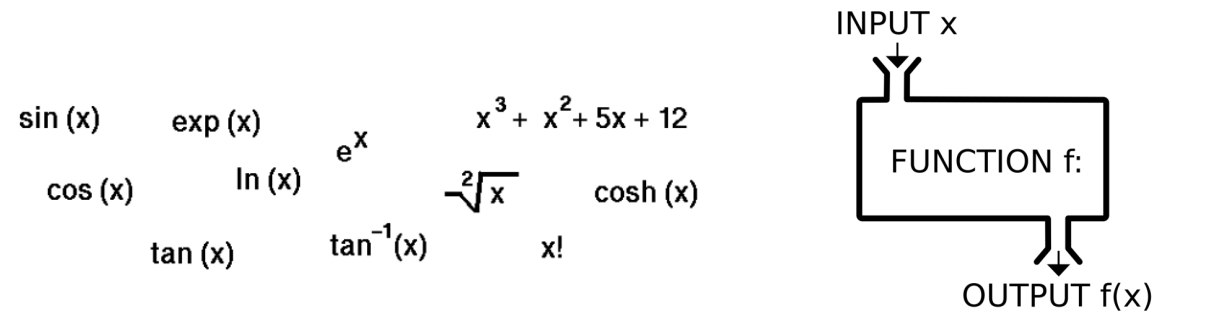
\includegraphics[width=0.5\textwidth]{reele-functie.png}
    \caption{Voorbeelden re"ele functies}
\end{figure}

\begin{theorem}
Voor elke functie geldt: er bestaat een \dots
    \begin{thmenum}
        \item \dots domein van de functie (domain)
        \item \dots beeld van de functie (range)
        \item \dots functievoorschrift van de functie
    \end{thmenum}
\end{theorem}

\begin{figure}[H]
    \centering
    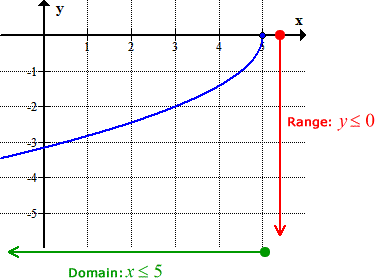
\includegraphics[width=0.5\textwidth]{functie-domain-range.png}
    \caption{Domein, bereik, functievoorschrift}
\end{figure}

$f: \mathbf{domein} \rightarrow \mathbf{bereik}: x \rightarrow y = f(x)$

$f: \mathbb{R} \rightarrow \mathbb{R} : x \rightarrow y = x^3 - 4x$

\begin{theorem}
    Elke functie kan nulpunten hebben.
\end{theorem}

\begin{figure}[H]
    \centering
    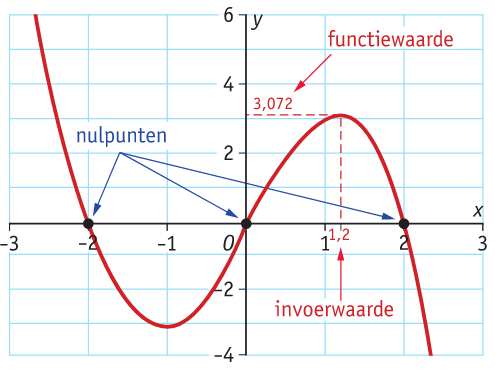
\includegraphics[width=0.5\textwidth]{functie-nulpunten.png}
    \caption{$y=-x^3 + 4x$}
\end{figure}

Verloop van een functie wordt via een tekenschema verduidelijkt:

\begin{figure}[H]
    \centering
    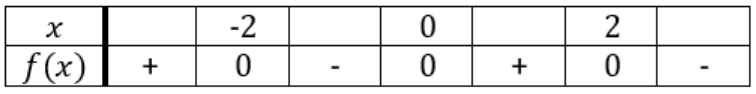
\includegraphics[width=0.5\textwidth]{functie-tekenschema.png}
    \caption{Tekenschema}
\end{figure}

\subsection{Veelterm en veeltermfuncties}

\begin{theorem}[Veelterm]
\begin{equation}
    \begin{aligned}
        A(x) = a_nx^n + a_{n-1}x^{n-1} + a_{n-2}x^{n-2} + ... + a_{2}x^{2} + a_1x + a_0\\
        (a_n,a_{n-1},...,a_2,a_1,a_0 \in \mathbb{R})
    \end{aligned}
\end{equation}

\end{theorem}

\begin{theorem}[Veeltermfunctie]
\begin{equation}
    \begin{aligned}
        f(x) = a_nx^n + a_{n-1}x^{n-1} + a_{n-2}x^{n-2} + ... + a_{2}x^{2} + a_1x + a_0\\
        Graad\ van\ veelterm = n\ als\ a_n \neq 0
    \end{aligned}
\end{equation}
\end{theorem}

\subsection{Bijzondere veeltermfuncties}

\begin{itemize}
    \item Constante functie: $f(x) = 4$
    \item Lineaire functie: $f(x) = 4$
    \item Tweedegraadsfunctie: $f(x) = 3x^2 + 2x + 1$
    \item Derdegraadsfunctie: $f(x) = 5x^3 - 3x^2 + 2x - 1$
    \item Exponenti"ele functie: $f(x) = 2^x$
    \item Logaritmische functie: $(fx) = log_2(x)$
\end{itemize}

\subsubsection{Constante functie}

\begin{figure}[H]
    \centering
    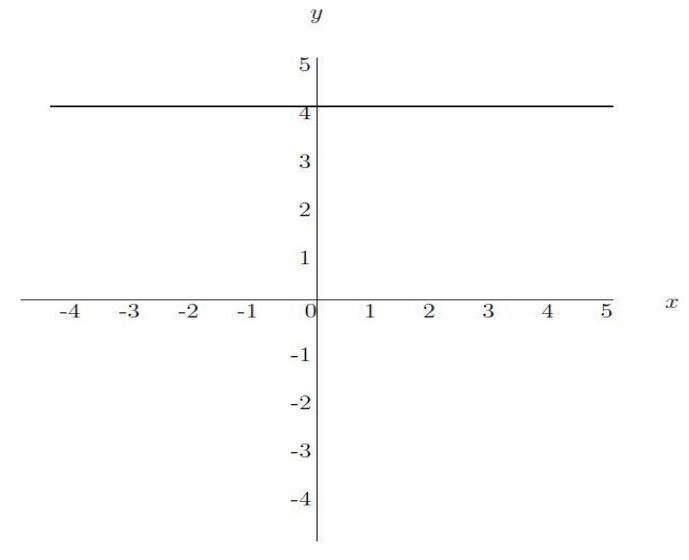
\includegraphics[width=0.3\textwidth]{functie-constant.png}
    \caption{$y=4$}
\end{figure}

\subsubsection{Lineaire functie}

\begin{theorem}[Lineaire functie]
    \begin{equation}
        f(x) = ax + b
    \end{equation}


Voorbeeld: $f(x) = 3x + 6$
\end{theorem}

\begin{itemize}
    \item Betekenis van a: de richtingsco"effici"ent (rico)
    \item Betekenis van b: het snijpunt met de y-as
    \item Nulpunt: TODO
\end{itemize}

\begin{figure}[H]
    \centering
    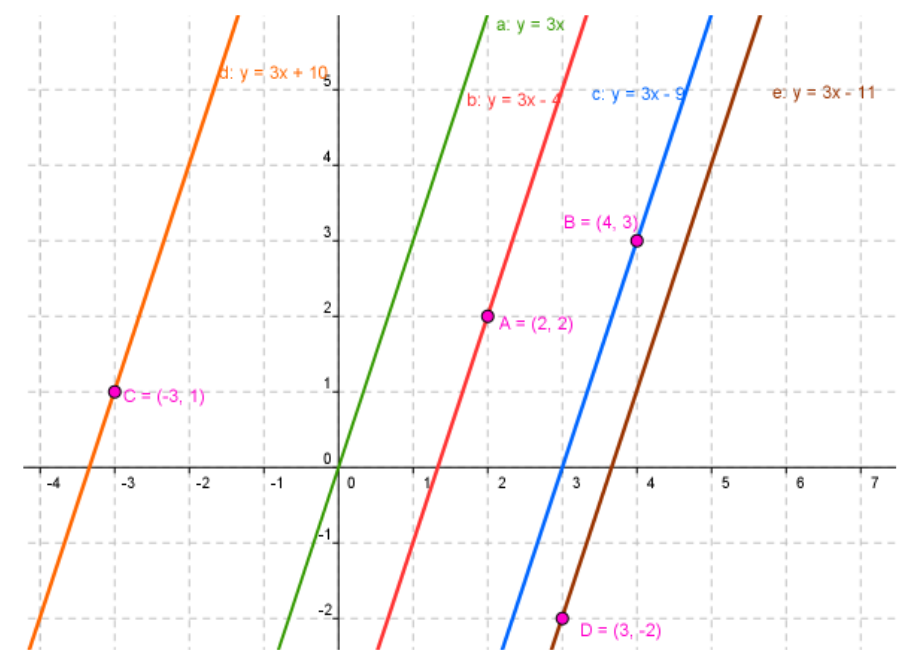
\includegraphics[width=0.3\textwidth]{functie-lineair2.png}
    \caption{Meerdere evenwijdige lineaire functies}
\end{figure}

Evenwijdige rechten als: als $a_1 = a_2$

Loodrechte rechten als: als $a_1 \cdot a_2 = -1$

\subsubsection{Tweedegraadsfunctie}

\begin{theorem}
\begin{equation}
    \begin{aligned}
        f(x) = ax^2 + bx + c,\\
        (a \neq 0)
    \end{aligned}
\end{equation}


\end{theorem}

\begin{figure}[H]
    \centering
    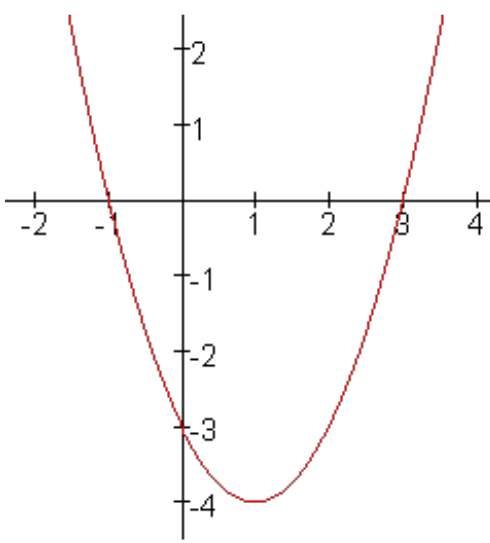
\includegraphics[width=0.2\textwidth]{functie-2degraad.png}
    \caption{$f(x) = x^2 - 2x - 3$}
\end{figure}

\begin{itemize}
    \item Betekenis van a: positief $\Rightarrow$ dalparabool, negatief $\Rightarrow$ bergparabool
    \item Nulpunten: via de discriminant berekenen:
\end{itemize}

\begin{theorem}[Discriminant]
Bij een tweedegraadsvergelijking is de discriminant:

\begin{equation}
    D = b^2 - 4ac
\end{equation}
\end{theorem}

\begin{itemize}
    \item Geval 1: $D > 0 \Rightarrow$ de functie heeft 2 nulpunten
    \item Geval 2: $D = 0 \Rightarrow$ de functie heeft 1 nulpunt
    \item Geval 3: $D < 0 \Rightarrow$ de functie heeft géén nulpunten
\end{itemize}

\begin{figure}[H]
    \centering
    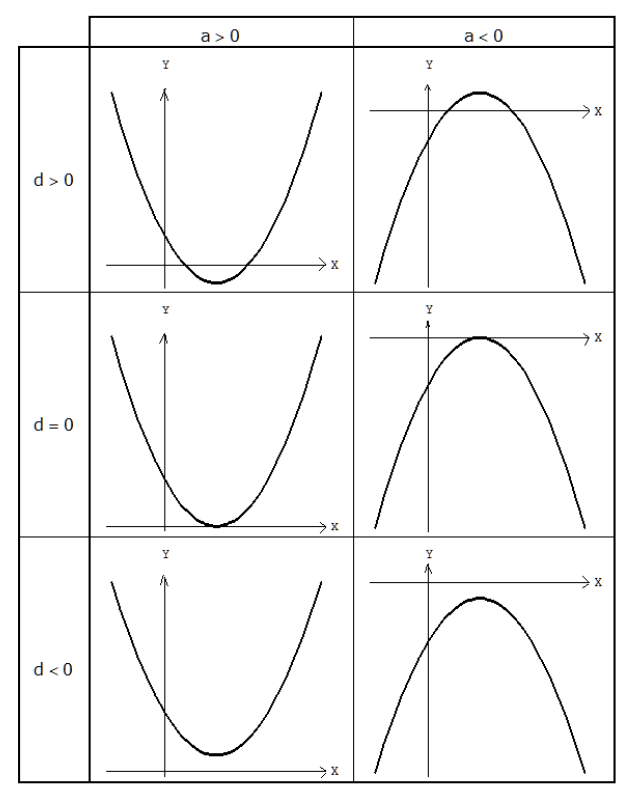
\includegraphics[width=0.4\textwidth]{functie-2degraad3.png}
    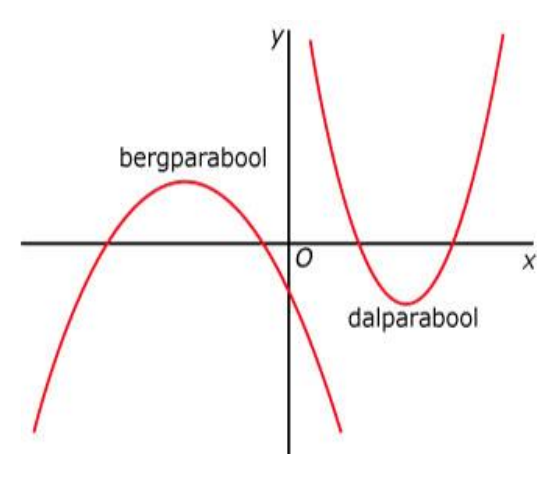
\includegraphics[width=0.3\textwidth]{functie-2degraad2.png}
    \caption{De discriminant toont de nulpunten}
\end{figure}

\textbf{Nulpunten berekenen:} 

\begin{equation}
    x_{1,2} = \frac{-b \pm \sqrt{D}}{2a}
\end{equation}

\begin{figure}[H]
    \centering
    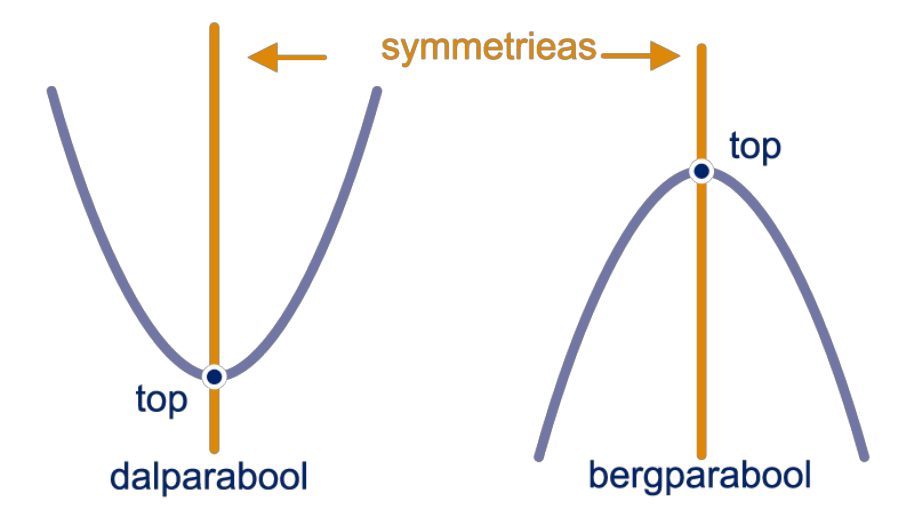
\includegraphics[width=0.5\textwidth]{functie-2degraad4.png}
    \caption{Symmetrieas: $x = \frac{-b}{2a}$}
\end{figure}

Voorbeeld: 

\begin{figure}[H]
    \centering
    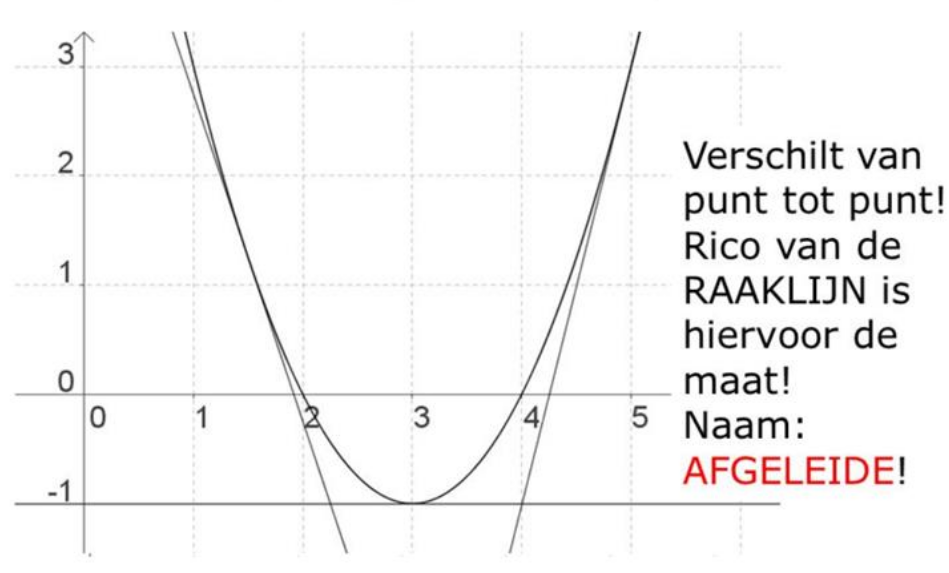
\includegraphics[width=0.5\textwidth]{functie-2degraad5.png}
    \caption{$y = x^2 - 6x + 8$}
\end{figure}

\subsubsection{Derdegraadsfunctie}

\begin{theorem}[Derdegraadsfunctie]
\begin{equation}
    \begin{aligned}
        f(x) = ax^3 + bx^2 + cx + d
        (a \neq 0)
    \end{aligned}
\end{equation}


\end{theorem}

\subsubsection{Exponenti"ele functie}

\begin{theorem}[Exponenti"ele functie]
\begin{equation}
    f(x) = a^{g(x)}
\end{equation}

Met grondtal $a \in \mathbb{R}_0^+ \backslash \{1\}$
\end{theorem}

\begin{figure}[H]
    \centering
    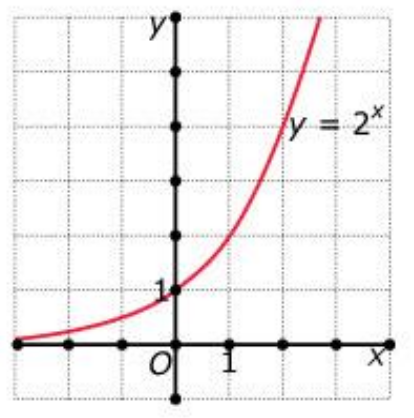
\includegraphics[width=0.3\textwidth]{functie-exponentieel.png}
    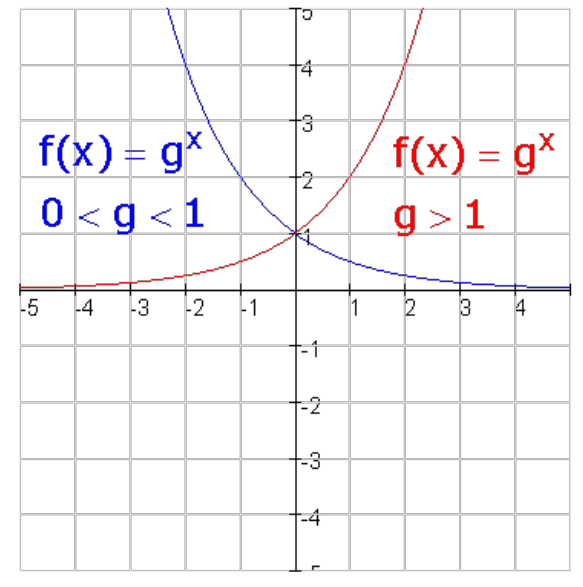
\includegraphics[width=0.3\textwidth]{functie-exponentieel2.png}
    \caption{}
\end{figure}


\begin{itemize}
    \item Betekenis van a: groeifactor
    \item Wanneer stijgend? 
    \item Wanneer dalend? 
    \item Nulpunten: 
    \item Vaststelling beeld functie
\end{itemize}



\begin{theorem}[Constante van Euler]

\begin{equation}
    \begin{aligned}
        e \approx 2.718281828\dots
    \end{aligned}
\end{equation}

$f(x) = e^x$ is een bijzondere exponenti"ele functie
\end{theorem}

\begin{figure}[H]
    \centering
    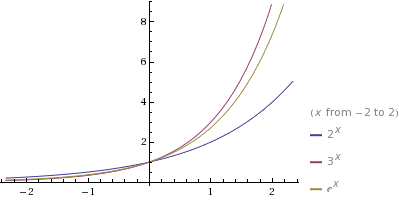
\includegraphics[width=0.5\textwidth]{functie-exponentieel3.png}
    \caption{Verschil tussen $2^x$, $3^x$ en $e^x$}
\end{figure}

\section{Exponenti"ele verbanden in data}

\subsection{Lineaire groei}

Kenmerkend:

\begin{itemize}
    \item Per tijdseenheid wordt hetzelfde getal \textbf{opgeteld}
    \item Grafiek is een rechte
    \item Algemene formule (N = aantal, t = tijd, b: beginhoeveelheid): 
    \begin{equation}
        N = a\cdot t + b
    \end{equation}
\end{itemize}

\begin{figure}[H]
    \centering
    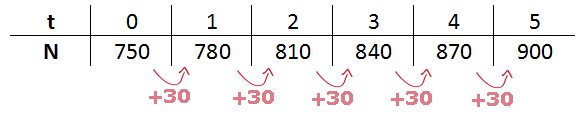
\includegraphics[width=0.5\textwidth]{lineaire-groei.png}
    \caption{Lineaire groei}
\end{figure}

\subsection{Exponenti"ele groei}

Kenmerkend: 

\begin{itemize}
    \item Per tijdseenheid wordt de hoeveelheid met hetzelfde getal \textbf{vermenigvuldigd}
    \item Grafiek is een exponenti"ele functie
    \item \textbf{Algemene formule:} 
    \begin{equation}
        N = b \cdot g^t
    \end{equation}
\end{itemize}

\begin{figure}[H]
    \centering
    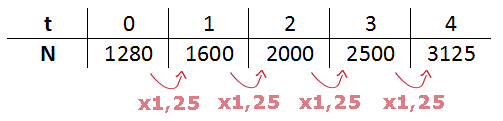
\includegraphics[width=0.5\textwidth]{exponentiele-groei.png}
    \caption{Exponenti"ele groei}
\end{figure}

\begin{figure}[H]
    \centering
    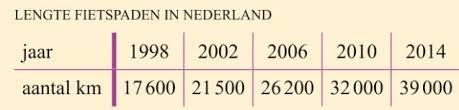
\includegraphics[width=0.5\textwidth]{voorbeeld-groei.png}
    \caption{Voorbeeld exponenti"ele groei met groeifactor $\approx 1.22$}
\end{figure}


\subsection{Van groeipercentage naar groeifactor}

De toename/afname wordt vaak ook procentueel uitgedrukt

\begin{itemize}
    \item Een jaarlijkse toename van $14.6\%$
    \item Een jaarlijkse afname van $14.6\%$
\end{itemize}

\begin{theorem}[Groeifactor]
De groeifactor is de factor die per tijdseenheid wordt vermenigvuldigd met de vorige waarde.
\end{theorem}

\subsubsection{Percentage naar factor}

\begin{equation}
g = \frac{p + 100}{100}\%
\end{equation} 

\begin{figure}[H]
    \centering
    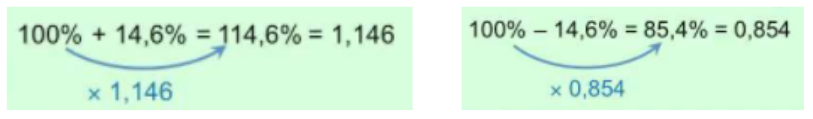
\includegraphics[width=0.5\textwidth]{percentage-naar-factor.png}
    \caption{Van groeipercentage naar groeifactor}
\end{figure}


\subsubsection{Factor naar percentage}

\begin{figure}[H]
    \centering
    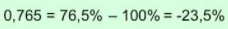
\includegraphics[width=0.35\textwidth]{factor-naar-percentage.png}
    \caption{Van groeifactor naar groeipercentage}
\end{figure}

\begin{figure}[H]
    \centering
    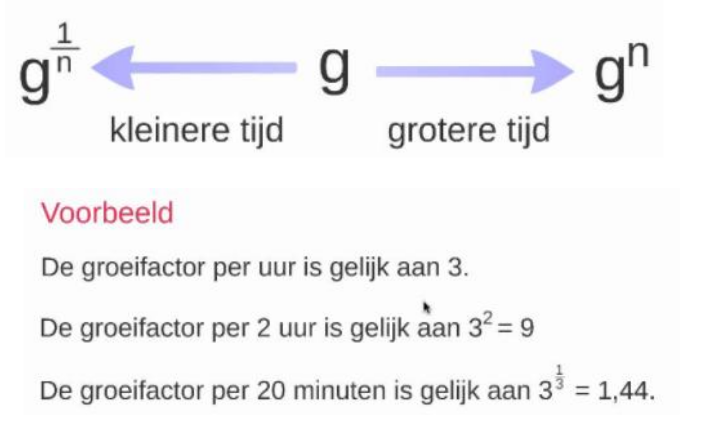
\includegraphics[width=0.5\textwidth]{groeifactoren.png}
    \caption{Let op: hier gebeuren vaak fouten bij het omrekenen}
\end{figure}

\subsection{Voorbeeld}

Een hoeveelheid groeit exponentieel. Na 5u is $N = 82$ en na 12u is $N = 246$.

Stel de formule van N op.

\textbf{Oplossing}

\begin{equation}
N = b \cdot g^t
\end{equation}

\underline{Stap 1: groeifactor berekenen per tijdseenheid:}

\begin{center}
$$
\left.
    \begin{array}{lll}
        \text{Na 5u}  & \rightarrow & N = 82 \\
        \text{Na 12u} & \rightarrow & N = 246 \\
    \end{array}
\right \} \Delta = 7u \rightarrow 164
$$


Groeifactor voor 7 uren: $\frac{246}{82} = 3$

Groeifactor voor 1 uur: $3^{1/7} \approx 1.170$
\end{center}

\underline{Stap 2: 1 punt nemen waarvan we N weten:}

\begin{center}

Gekozen punt: $(5, 82)$

$82 = b \cdot (1.170)^5$

$\Leftrightarrow b = \frac{82}{1.170}^5 \approx 37$

$\Leftrightarrow N = 37 \cdot 1.170^t$
\end{center}

\subsection{Belangrijke maten voor exponenti"ele toename}


\begin{theorem}[Verdubbelingstijd]
De verdubbelingstijd is de nodige tijd tot de hoeveelheid verdubbeld is.

De verdubbelingstijd $t$ kan je berekenen met:
\begin{equation}
g^t = 2
\end{equation}
\end{theorem}

\textbf{Oefening}

De populatie neemt toe met $8.3\%$ per jaar. Bereken de verdubbelingstijd:

\begin{center}
$g^t = 2$

$\Leftrightarrow (1.083)^t = 2$

$\Leftrightarrow \log(1.083^t) = \log(2)$

$\Leftrightarrow t \cdot \log(1.083) = \log(2)$

$\Leftrightarrow t = \frac{\log(2)}{\log(1.083)}$

$\Leftrightarrow t = 8.69\ jaar$

\end{center}


\begin{theorem}[Halveringstijd]
De halveringstijd is de nodige tijd tot de hoeveelheid gehalveerd is.

De halveringstijd $t$ kan je berekenen met:
\begin{equation}
g^t = 1/2
\end{equation}
\end{theorem}

\subsubsection{Oefening: Combinatie van groeifactoren?}

Een hoeveelheid neemt eerst 5 jaar lang met vast percentage (*) toe, 
om daarna nog 3 jaar met 10\% per jaar toe te nemen. Na 8 jaar is
de totale hoeveelheid verdubbeld.

(*) Bereken het jaarlijkse groeipercentage in de eerste 5 jaren.

\textbf{Oplossing}

We weten:

\begin{itemize}
    \item Eerste 5 jaar: toename met vast percentage
    \item Volgende 3 jaar: toename met 10\% (= factor van 1.1)
    \item Na 8 jaar: hoeveelheid verdubbeld (= factor van 2)
\end{itemize}

\begin{center}
$g^5 \cdot 1.1^3 = 2$

We moeten $g$ vinden:

$\Leftrightarrow g^5 = \frac{2}{1.1^3}$

$\Leftrightarrow g = \sqrt[5]{\frac{2}{1.1^3}}$
\end{center}



\end{document}